\documentclass[aspectratio=169]{../latex_main/tntbeamer}  % you can pass all options of the beamer class, e.g., 'handout' or 'aspectratio=43'
\usepackage{dsfont}
\usepackage{bm}
\usepackage[english]{babel}
\usepackage[T1]{fontenc}
%\usepackage[utf8]{inputenc}
\usepackage{graphicx}
\graphicspath{ {./figures/} }
\usepackage{algorithm}
\usepackage[ruled,vlined,algo2e,linesnumbered]{algorithm2e}
\usepackage{hyperref}
\usepackage{booktabs}
\usepackage{mathtools}

\usepackage{amsmath,amssymb}

\DeclareMathOperator*{\argmax}{arg\,max}
\DeclareMathOperator*{\argmin}{arg\,min}

\usepackage{amsbsy}
\newcommand{\vect}[1]{\bm{#1}}
%\newcommand{\vect}[1]{\boldsymbol{#1}}

\usepackage{pgfplots}
\pgfplotsset{compat=1.16}
\usepackage{tikz}
\usetikzlibrary{trees} 
\usetikzlibrary{shapes.geometric}
\usetikzlibrary{positioning,shapes,shadows,arrows,calc,mindmap}
\usetikzlibrary{positioning,fadings,through}
\usetikzlibrary{decorations.pathreplacing}
\usetikzlibrary{intersections}
\pgfdeclarelayer{background}
\pgfdeclarelayer{foreground}
\pgfsetlayers{background,main,foreground}
\tikzstyle{activity}=[rectangle, draw=black, rounded corners, text centered, text width=8em]
\tikzstyle{data}=[rectangle, draw=black, text centered, text width=8em]
\tikzstyle{myarrow}=[->, thick, draw=black]

% Define the layers to draw the diagram
\pgfdeclarelayer{background}
\pgfdeclarelayer{foreground}
\pgfsetlayers{background,main,foreground}

% Requires XeLaTeX or LuaLaTeX
%\usepackage{unicode-math}

\usepackage{fontspec}
%\setsansfont{Arial}
\setsansfont{RotisSansSerifStd}[ 
Path=../latex_main/fonts/,
Extension = .otf,
UprightFont = *-Regular,  % or *-Light
BoldFont = *-ExtraBold,  % or *-Bold
ItalicFont = *-Italic
]
\setmonofont{Cascadia Mono}[
Scale=0.8
]

% scale factor adapted; mathrm font added (Benjamin Spitschan @TNT, 2021-06-01)
%\setmathfont[Scale=1.05]{Libertinus Math}
%\setmathrm[Scale=1.05]{Libertinus Math}

% other available math fonts are (not exhaustive)
% Latin Modern Math
% XITS Math
% Libertinus Math
% Asana Math
% Fira Math
% TeX Gyre Pagella Math
% TeX Gyre Bonum Math
% TeX Gyre Schola Math
% TeX Gyre Termes Math

% Literature References
\newcommand{\lit}[2]{\href{#2}{\footnotesize\color{black!60}[#1]}}

%%% Beamer Customization
%----------------------------------------------------------------------
% (Don't) Show sections in frame header. Options: 'sections', 'sections light', empty
\setbeamertemplate{headline}{empty}

% Add header logo for normal frames
\setheaderimage{
	% 
\includegraphics[height=\logoheight]{figures/TNT_darkv4.pdf}
	
\includegraphics[height=\logoheight]{../latex_main/figures/luh_logo_rgb_0_80_155.pdf}
	% 
\includegraphics[height=\logoheight]{figures/logo_tntluh.pdf}
}

% Header logo for title page
\settitleheaderimage{
	% 
\includegraphics[height=\logoheight]{figures/TNT_darkv4.pdf}
	
\includegraphics[height=\logoheight]{../latex_main/figures/luh_logo_rgb_0_80_155.pdf}
	% 
\includegraphics[height=\logoheight]{figures/logo_tntluh.pdf}
}

% Title page: tntdefault 
\setbeamertemplate{title page}[tntdefault]  % or luhstyle
% Add optional title image here
%\addtitlepageimagedefault{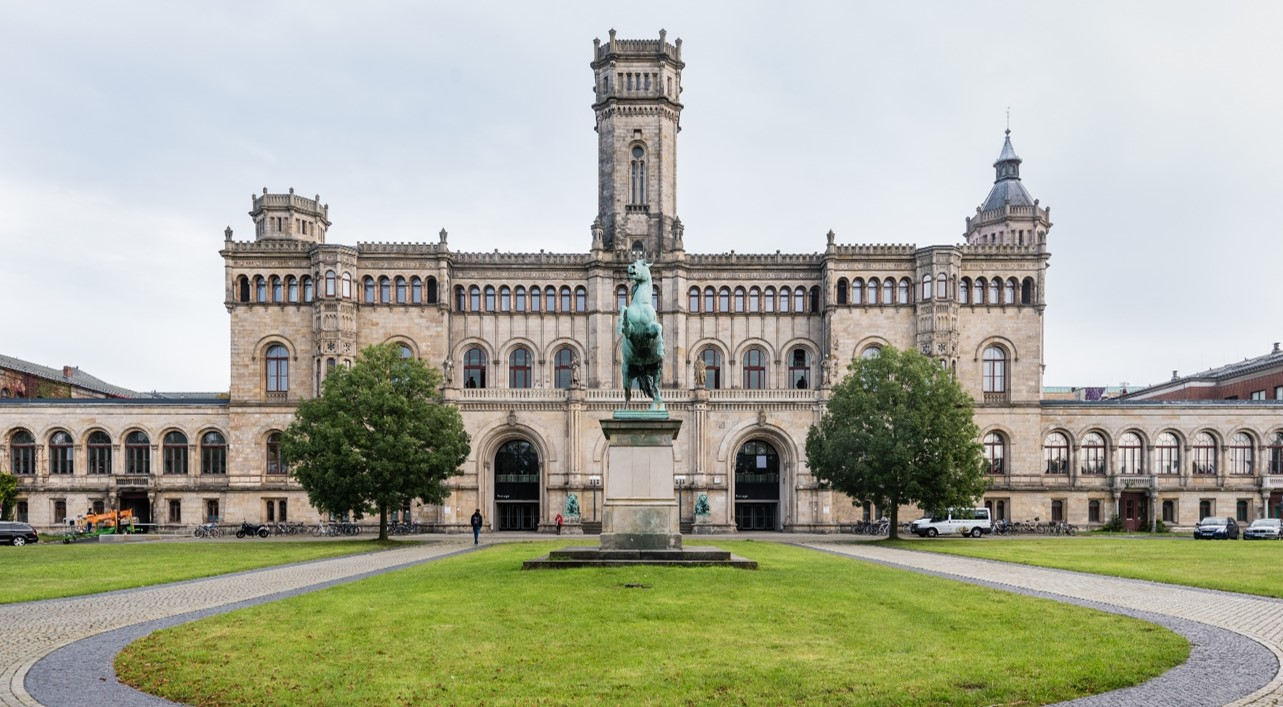
\includegraphics[width=0.65\textwidth]{figures/luh_default_presentation_title_image.jpg}}

% Title page: luhstyle
% \setbeamertemplate{title page}[luhstyle]
% % Add optional title image here
% \addtitlepageimage{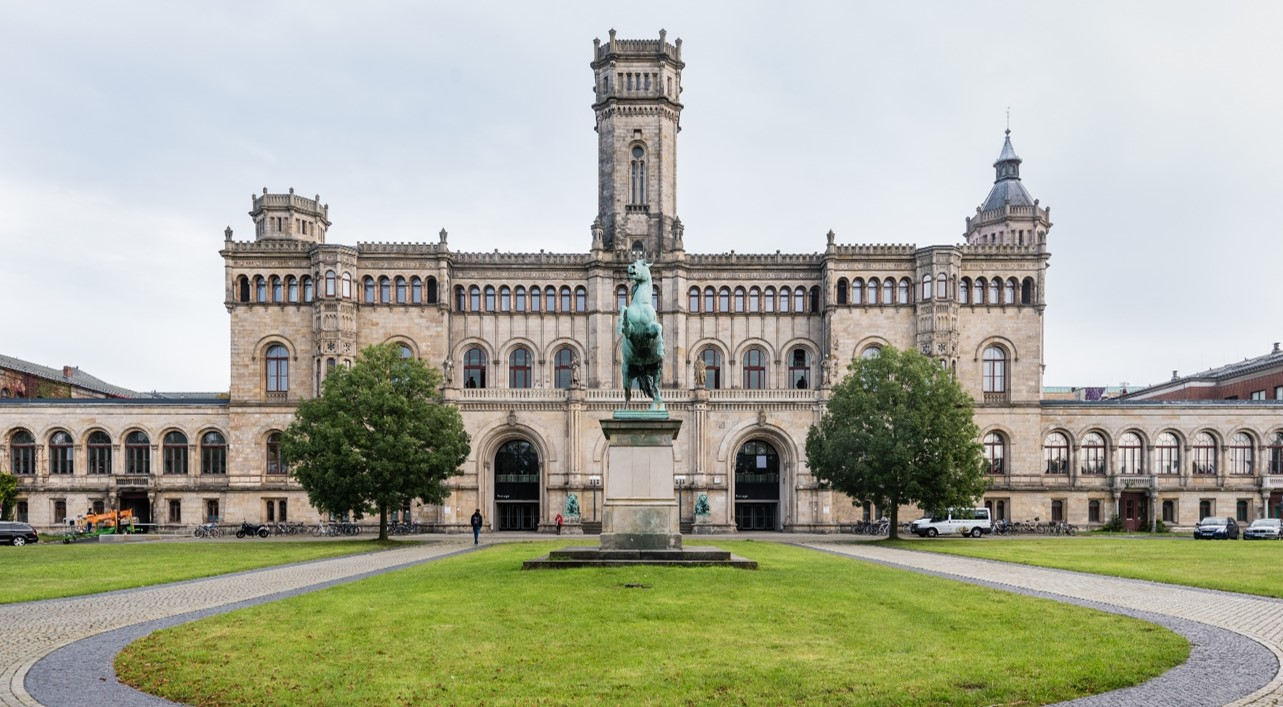
\includegraphics[width=0.75\textwidth]{figures/luh_default_presentation_title_image.jpg}}

\author[Abedjan \& Lindauer]{Ziawasch Abedjan \& Marius Lindauer\\[1em]
	
\includegraphics[height=\logoheight]{../latex_main/figures/luh_logo_rgb_0_80_155.pdf}\qquad
	
\includegraphics[height=\logoheight]{../latex_main/figures/DBIS_Kurzlogo.png}\qquad

\includegraphics[height=\logoheight]{../latex_main/figures/TNT_darkv4}\qquad

\includegraphics[height=\logoheight]{../latex_main/figures/L3S.jpg}	}
\date{Summer Term 2022; \hspace{0.5em} {
\includegraphics[height=1.5em]{../latex_main/figures/Cc-by-nc-sa_icon.svg.png}}; based on \href{https://ds100.org/fa21/}{[DS100]}
}


%%% Custom Packages
%----------------------------------------------------------------------
% Create dummy content
\usepackage{blindtext}

% Adds a frame with the current page layout. Just call \layout inside of a frame.
\usepackage{layout}


%%% Macros
%\renewcommand{\vec}[1]{\mathbf{#1}}
% \usepackage{bm}
%\let\vecb\bm

\title[Statistics]{DS: Bias and Variance}
\subtitle{Expectation, Revisited}

\graphicspath{ {./figure/} }
%\institute{}


\begin{document}
	
	\maketitle
	\begin{frame}{Random Variable (RV)}
	    \begin{columns}
	        \begin{column}{.4\textwidth}
	                A random variable is a variable that can takes numerical values with particular probabilities.\\
	                \bigskip
	                Example 1:\\
                    Let $X$ take the value $1$ if FDR, $0$ if \\
                    Landon\\
                    \bigskip
                    Example 2:\\
                    Let $Y$ be the \# of pips on a roll of a \\
                    6-sided die



	        \end{column}
	        
	        
	        \begin{column}{.4\textwidth}
	            Notation:
	                \begin{itemize}
	                    \item Random variables (RVs) use capital letters
	                    \begin{itemize}
	                        \item $X$, $Y$, $Z$
	                    \end{itemize}
	                    \item A particular value taken by an RV is indicated by a lowercase letter.
	                    \begin{itemize}
	                        \item $x$, $y$, $z$
	                    \end{itemize}
	                    \item The (Probability) Distribution of a discrete RV can be expressed as a table or graphic.
	                    \begin{itemize}
	                        \item $P(X = x)$
	                    \end{itemize}
	                \end{itemize}
	        \end{column}
	    \end{columns}
	\end{frame}
	
	
	\begin{frame}[c]{Discrete vs. Continuous}
	    
	   \vspace{-2em}
	    \begin{columns}
	    
	        \begin{column}{.5\textwidth}
	        
	           \begin{itemize}
	               \item Focus on discrete distributions so far 
	               \item Discrete RVs:
	               \begin{itemize}
	                   \item can only take on specific values
	                   \item defined by their Probability Mass Function
	               \end{itemize}
	               \item Example: Binomial Distribution.
	           \end{itemize}
                        \centering
                        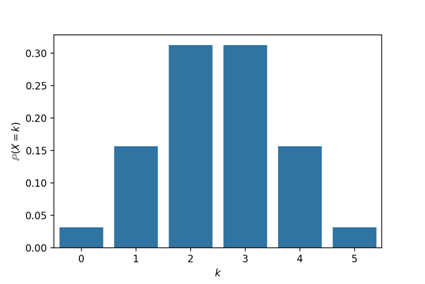
\includegraphics[scale=.5]{Bild4}
                        
	        \end{column}
	        
	        \begin{column}{.5\textwidth}
	        
	                \begin{itemize}
	                    \item RVs can also follow continuous distributions
	                    \item For example, $\epsilon$ in our data generation process
	                    \item Continuous RVs 
	                    \begin{itemize}
	                        \item can take values to arbitrary precision
	                        \item defined by their Probability Density Function (PDF)
	                    \end{itemize}
	                    \item Example: Gaussian Distribution.\\
	                \end{itemize}
	                
	                    \centering
                        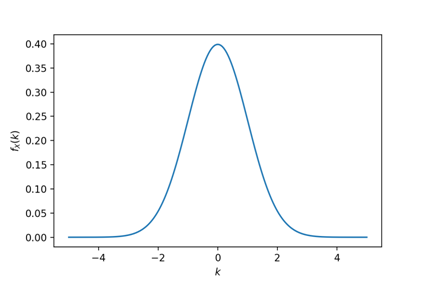
\includegraphics[scale=.5]{Bild5}
	        \end{column}
	    \end{columns}
	\end{frame}
	
	
	\begin{frame}{Expectations for Discrete RVs}
	
	    The expectation of a random variable $X$ is the weighted average of the values of $X$, where the weights are the probabilities of the values.
	    
	    \begin{equation}
	        \mathbb{E}(X) =  \sum_{x_i} P(X= x_i) \cdot x_i \nonumber
	    \end{equation}
	    
	    \begin{itemize}
	        \item P(X) could follow different discrete distributions in the above case (e.g., Bernoulli or Binomial)
	    \end{itemize}

	    \begin{itemize}
	                \item Expectation is a number, not a random variable
	                \item It is analogous to the average.
	                \begin{itemize}
	                    \item It has the same units as the random variable.
	                    \item It doesn’t need to be a possible value of the random variable.
	                    \item It is the center of gravity of the probability histogram.
	                \end{itemize}
	    \end{itemize}

	\end{frame}
	
	\begin{frame}{Expectations for Continuous RVs}
	
        Discrete RV:
	    \begin{equation}
	        \mathbb{E}(X) =  \sum_{x_i} P(X= x_i) \cdot x_i \nonumber
	    \end{equation}
	    
	    Continuous RV:
	    \begin{equation}
	        \mathbb{E}(X) =  \int^{\infty}_{-\infty} f(x_i) \cdot x_i \nonumber
	    \end{equation}
	    
	    \begin{itemize}
	        \item where f is the probability density function (PDF)
	        \item Same idea to weight each $x_i$ by the PDF
	        \item \alert{Warning}: 
	        \begin{itemize}
	            \item $f$ is not a probability, i.e., not bounded in [0,1]
	            \item a specific $x_i$ has a probability of close to $0$
	            \item $\int^{U}_{-\infty} f(x_i) \cdot x_i$ provides $P(X<U)$
	        \end{itemize}
	        
	    \end{itemize}
	    
	\end{frame}
	
	
	
	\begin{frame}[c]{Properties of Expectations}
	    Linear transformations\\
	    Let $Z = aX + b;\hspace{5mm} \mathbb{E}(Z) = \mathbb{E}( aX + b) = a\mathbb{E}(X) + \mathbb{E}(b) = a\mathbb{E}(X) + b$
	    
	    where $a$ and $b$ are constants\\[2em]
	    
	    Additivity\\
	    Let $W = X_1 + X_2; \hspace{5mm} \mathbb{E}(W) = \mathbb{E}( X_1 + X_2) =  \mathbb{E}( X_1) + \mathbb{E}(X_2)$\\[2em]

	    Linearity of Expectation\\
	    Let $V = aX_1 + bX_2;\hspace{5mm} \mathbb{E}(V) = \mathbb{E}( aX_1 + bX_2) = a\mathbb{E}(X_1) + b\mathbb{E}(X_2)  $
	\end{frame}
	
	
	\begin{frame}[c]{Expectation of a Function of a Random Variable}
	    What if we want to calculate $E(X^2)$? Or more generally, $\mathbb{E}(f(X))$? Does $\mathbb{E}(f(X))$ equal $f( \mathbb{E}(X) )$? \alert{No!}
	    
	    Let’s work through an example with the distribution of one six-sided die roll:
	    \begin{align*}
	        \mathbb{E}(f(x)) &= \sum\limits_kf(k){P}(X=k)\\
	        \mathbb{E}(X^2) &= \sum\limits_kk^2{P}(X=k)\\
	        &= 1^2\cdot \frac{1}{6} + 2^2\cdot \frac{1}{6} + 3^2\cdot \frac{1}{6} + 4^2\cdot \frac{1}{6} +  5^2\cdot \frac{1}{6} + 6^2\cdot \frac{1}{6} = \frac{91}{6}\\
	        \mathbb{E}(X^2) &\neq (\mathbb{E}(X))^2 = \left(\frac{7}{2}\right)^2 = \frac{49}{4}
	    \end{align*}
	\end{frame}
	
	
	\begin{frame}[c]{Estimators and Bias}
	    Recall that parameters represent the truth, and we estimate these parameters with statistics\\
	    Take the function: $g(x) = \theta_0 + \theta_1x$\\
	   $\theta_0$ and $\theta_1$ are parameters. We estimate them with:
	    \begin{align*}
	       \hat{\theta}_1 = r\frac{\sigma_y}{\sigma_x}\hspace{5mm} \hat{\theta}_0 = \overline{y} - \hat{\theta}_1\overline{x}
	    \end{align*}
	    Recall that statistical bias is the expected difference between your estimate and the truth.
        \begin{align*}
            \mathbb{E}(\hat{\theta} - \theta) = \mathbb{E}(\hat{\theta}) - \theta
        \end{align*}
        Remember, $\hat{\theta}$	is random! It is random because the dataset you sample is random.\\
        (It can be proven that the above estimates for $\theta_0$ and $\theta_1$ are unbiased.)

	\end{frame}
	
	
	\begin{frame}[c]{Summary}
	   \begin{itemize}
	       \item Random variables are functions of our sample.
	       \item The expectation of a random variable is the weighted average of its possible values, weighted by the probabilities of those values.
	       \begin{itemize}
	           \item Expectation behaves nicely with linear transformations of random variables.
	           \item Expectation is also additive.
	           \item We can calculate the expectation of a function of a random variable.
	       \end{itemize}
	       \item The optimal weights in our linear models are estimates of the true parameters.
	   \end{itemize}
	\end{frame}
\end{document}